\documentclass{article}
\title{Assignment \bf{ Mice }}
\date{31.07.2013}
\usepackage[english]{babel}
\usepackage[cp1250]{inputenc}
\usepackage{hyperref}
\usepackage{enumerate}
\usepackage[cm,empty]{fullpage}
\usepackage[pdftex]{graphicx,color}
\usepackage{Sweave}
\begin{document}
\maketitle{}
\section{ Data about the group }{\bf : }Mickey Mouse, Minnie Mouse, Morty Fieldmouse, Ferdie Fieldmouse\\{\bf Due date : 1st of October 2012 }\\{\bf Sources : }Lecture Notes\\{\bf Template to use : Descriptive.doc }\\\section{ Assignment }Answer to the following questions \\\begin{itemize}
\item Calculate the mean of the following data: 
 
-3,0,7,12 
\item Calculate the standard deviation of the following data:  

7,-5,-10,15 
\item Data for the  variable nn are represented graphically. Determine (approximately) the mean and the standard deviation of the variable.\\ 
\begin{tabular}{c}
\resizebox{50mm}{!}{

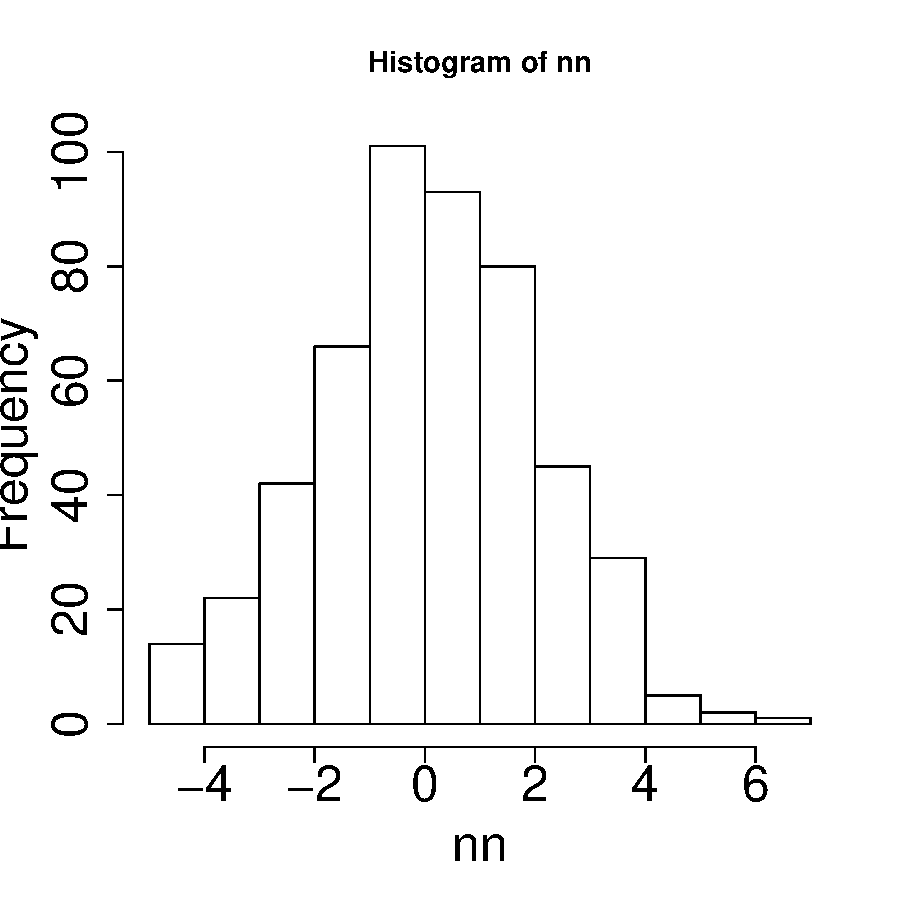
\includegraphics{Mice-003}
}
\end{tabular} 
\end{itemize}
\vspace{\baselineskip} {\bf Good luck! }\newpage
\end{document}
